\scanpage{530}
% E530-01
\mspage{568}
\uline{$\overline{\mathrm{IV}}$}\quad
% E530-02
\deleted{Soit}

% E530-03
Soit donc $\mathcal{G}$ un groupe profini, muni \unsure{des|de}
% E530-04
\inserted{générateurs}
$\rho,\sigma\in\mathcal{G}$ satisfaisant les relations
% E530-05
\[
(1)\qquad \rho^6=\sigma^4=1,\qquad
\rho^3=\sigma^2\quad (\overset{\mathrm{dfn}}{=}\text{``$-1$''}) .
\]
% E530-06
\margin{Ceci signifie simplement qu'on se donne un hom. surjectif
% E530-07
\diagram{\begin{tikzcd}[ampersand replacement=\&]
\mathrm{SL}(2,\mathbb Z)^{\wedge}\arrow[r] \& \mathcal{G}
\end{tikzcd}}}

% E530-08
Un cas particulièrement intéressant est celui où
$\rho^3=\sigma^2=1$, auquel néanmoins \unsure{je} ne
\unsure{voudrais} me limiter. Soit $\tau$ un \unsure{autom.}
de $\mathcal{G}$ satisfaisant
% E530-09
\[
(2)\qquad
\tau(\deleted{\unsure{\rho}}\inserted{\sigma})=
\begin{array}{c}\sigma^{-1}\\[-2pt]\inserted{=-\sigma}\end{array},
\qquad \tau(\rho)=\sigma(\rho^{-1})
\]
% E530-10
\margin{Introduisons \deleted{\unsure{le}} de suite l'élément
\unsure{équivalent} $\tau'=\sigma^{-1}\tau$ satisfaisant
$\tau'(\rho)=\rho^{-1}$, $\tau'(\sigma)=\sigma^{-1}$
$(\tau'(\varepsilon_0)=\varepsilon_1^{-1},\tau'(\varepsilon_1)=\varepsilon_0^{-1})$.}
% E530-11
(ce qui signifie que $\tau_\infty$ ``passe au quotient'' en un
\unsure{autom.} $\tau$ de $\mathcal{G}$), ce qui implique
% E530-12
\[
(3)\qquad \tau^2=1
\]
% E530-13
\[
(4)\qquad \tau(\varepsilon_0)=\varepsilon_0^{-1},\qquad
\tau(\varepsilon_1)=\varepsilon_1^{-1},\qquad\text{où}
\]
% E530-14
\[
(5)\qquad
\begin{array}{c}
\varepsilon_0=\deleted{\unsure{\alpha}}\sigma\rho\\[-2pt]
\inserted{=-\sigma^{-1}\rho}
\end{array},\qquad
\varepsilon_1=\rho\sigma=\sigma(\varepsilon_0)
=\sigma^{-1}(\varepsilon_0)=\rho(\varepsilon_0).
\]
% E530-15
\margin{\unsure{du form.}\ \unsure{oublié}\ \unsure{un} signe $-$,
alors \unsure{qu'on pourrait} \unsure{d'emblée|demander}
simplement \unsure{donner|prendre}
$\varepsilon_0=\unsure{\sigma_\infty|\sigma^{-1}}\rho\ldots$}

% E530-16
Posons
% E530-17
\[
(5)\qquad \mathcal{G}'=\{1,\tau\}\mathbin{.}\mathcal{G},
\]
% E530-18
donc on a
% E530-19
\[
(6)\qquad
\diagram{\begin{tikzcd}[ampersand replacement=\&]
1\arrow[r]\&\mathcal{G}\arrow[r]\&\mathcal{G}'\arrow[r]\&
\{1,\tau\}\arrow[r]\&1.
\end{tikzcd}}
\]

% E530-20
Soit
% E530-21
\deleted{\unsure{(7)}}
% E530-22
\[
\begin{gathered}
B_{\rho,\sigma}\subset\operatorname{Aut}(\mathcal{G})\times\widehat{\mathbb Z}^{*}
\\
(7)\qquad =\left\{(u,\mu)\ \left|\
\begin{array}{l}
u(\varepsilon_0)=\varepsilon_0^\mu\\
\deleted{\text{et}}\ u(\sigma)\ \text{conjugué dans }\mathcal{G}\text{ à }\sigma^\mu\\
u(\rho)\quad\rule{4cm}{0.3pt}\quad
\mathcal{G}^{\deleted{\unsure{\prime}}}\text{ à }\rho^\mu
\end{array}\right.\right\}.
\end{gathered}
\]
% E530-23
qui est évidemment un \uline{sous-groupe}.
La troisième condition \unsure{s'explicite} d'ailleurs,
% E530-24
\margin{529}

% E530-F01
\margin{\begin{center}
529\\
\texttt{https://grothendieck.umontpellier.fr}\\
Université de Montpellier, UMR CNRS 5149, Case courrier 051, Place Eugène Bataillon\\
34095 Montpellier cedex 5 - France
\end{center}}

\scanpage{531}
% E531-01
puisque $\rho^6=1$ i.e. $\rho^\mu$ ne dépend que de l'image
de $\mu$ dans
% E531-02
\[
(\mathbb Z/6\mathbb Z)^*\simeq
\inserted{(\mathbb Z/2\mathbb Z)^*\times}
(\mathbb Z/3\mathbb Z)^*\simeq(\mathbb Z/3\mathbb Z)^*\simeq\pm1,
\]
% E531-03
\deleted{\unsure{que} de \illegible{1}}
% E531-04
\inserted{donc}
% E531-05
\[
(8)\qquad \rho^\mu=\rho^{\varepsilon_3(\mu)}
\]
% E531-06
que pour $\varepsilon_3(\mu)=1$
% E531-07
\deleted{on}
$u(\rho)$ est conjugué à $\rho$ dans $\mathcal{G}$, et pour
$\varepsilon_3(\mu)=-1$ il est conjugué à $\rho^{-1}$ dans
$\mathcal{G}$, ou encore à $\rho$ par un élément de
$\mathcal{G}'$ -- i.e. un élément de la forme $\alpha_1\tau_\infty$
avec $\alpha_1\in\mathcal{G}$ (puisque
$\tau_\infty(\rho)=\inserted{\sigma}(\rho^{-1})$ justement\ldots).
% E531-08
\deleted{On aura donc,}
% E531-09
\deleted{\[
(9)\qquad u(\rho)=\zeta\rho,\qquad u(\sigma)=\eta\sigma
\quad(\zeta,\eta\in\mathcal{G})
\]}
% E531-10
\deleted{des relations}
% E531-11
\deleted{\[
(10)\qquad \zeta=\alpha\rho(\alpha)^{-1},
\qquad\eta=\beta
\]}
% E531-12
On voit de $\overline{\mathrm m}$ qu'on a
% E531-13
\[
\begin{aligned}
(9)\qquad \sigma^\mu=\sigma^{\varepsilon_2(\mu)}
&\quad\left\{\begin{array}{ll}
=\sigma&\text{si }\mu\equiv1\quad(4)\\
\deleted{\unsure{=}}\sigma^{-1}=-\sigma
&\text{si }\mu\equiv-1\quad(4)
\end{array}\right.\\[-2pt]
&\hspace{2.5cm}\deleted{=\unsure{\varepsilon\sigma|\sigma}}\\
&=\varepsilon_2(\mu)\sigma
\end{aligned}
\]
% E531-14
\deleted{Mais Donc $\unsure{\overline{\mathrm m}|=}$ \unsure{nous écrivons}
(pour $(u,\mu)\in B_{\rho,\sigma}$) des
\deleted{\unsure{tels $\alpha\in$}} éléments
$\alpha\in\mathcal{G}'$, $\beta\in$}

% E531-15
Ainsi :

% E531-16
\uline{Proposition}\quad Pour \unsure{qu'un|qu'on}
% E531-17
\deleted{ait}
$(u,\mu)\in\operatorname{Aut}
(\deleted{\unsure{B_{\rho,\sigma}}}\inserted{\mathcal{G}})
\times\widehat{\mathbb Z}^{*}$ soit dans $B_{\rho,\sigma}$,
il f. et s. qu'il existe
$\alpha\in\mathcal{G}'_{\deleted{\unsure{\rho,\sigma}}}
{}^{\deleted{\unsure{\varepsilon_3}}}$,
$\beta\in\mathcal{G}$ tels qu'on ait
% E531-18
\margin{530}

% E531-F01
\margin{\begin{center}
530\\
\texttt{https://grothendieck.umontpellier.fr}\\
Université de Montpellier, UMR CNRS 5149, Case courrier 051, Place Eugène Bataillon\\
34095 Montpellier cedex 5 - France
\end{center}}

\scanpage{532}
% E532-01
\mspage{569}
% E532-02
\[
(10)\qquad \unsure{u}(\rho)=\operatorname{int}(\alpha)(\rho),\qquad
u(\sigma)=\underbrace{\varepsilon_2(\mu)}_{\varepsilon}
\operatorname{int}(\beta)(\sigma)
\]
% E532-03
et enfin
% E532-04
\[
(11)\qquad u(\varepsilon_0)=\varepsilon_0^\mu,
\]
% E532-05
où de plus on a
% E532-06
\deleted{\[
(12)\qquad
\alpha\overset{\inserted{\in\mathcal{G}}}{\unsure{\bmod}\mathcal{G}}
\equiv\tau^{\overset{\inserted{\unsure{\nu_3}}}
{\unsure{\varepsilon_3(\mu)}}}
\quad\overset{\inserted{\mu\equiv1\ (3)}}{(\mathcal{G})}
\quad\text{i.e. }\alpha\in\mathcal{G}\unsure{\Longleftrightarrow}\mu.
\]}
% E532-07
\margin{i.e. $\unsure{\alpha}\equiv\tau$.}

% E532-08
On notera que
% E532-09
\deleted{$u$}\inserted{$(u,\mu)$}
est uniquement déterminé par
% E532-10
\inserted{$\mu$ et}
la connaissance de $\alpha$
% E532-11
\inserted{et}
de $\beta$,
% E532-12
\deleted{et de $\varepsilon_2(\mu)$}
et $\overline{\mathrm m}$ \unsure{seulement} par $\mu$ et
% E532-13
\[
(13)\qquad \zeta=\alpha\rho(\alpha)^{-1},\qquad
\eta=\varepsilon_2(\mu)\beta\sigma(\beta)^{-1}
\]
% E532-14
puisqu'on \unsure{aura alors} $u$ par
% E532-15
\[
(14)\qquad u(\rho)=\zeta\rho,\qquad u(\sigma)=\eta\sigma.
\]

% E532-16
D'ailleurs, dans le cas où
% E532-17
\[
(15)\qquad
\diagram{\begin{tikzcd}[ampersand replacement=\&]
\widehat{\mathbb Z}\arrow[r]\&\mathcal{G}\\
n\arrow[r,mapsto]\&\varepsilon_0^n
\end{tikzcd}}
\]
% E532-18
est injectif,
% E532-19
\deleted{alors}
$\mu$ est déterminé en fonction de $u$ comme
% E532-20
\inserted{multiplicateur de}
l'action de
% E532-21
\deleted{\unsure{$u$}}\inserted{$u$}
sur $L_0^{\mathcal{G}}\subset\mathcal{G}$, image de (15),
donc $(u,\mu)$ est déterminé par $u$ donc par
$(\alpha,\beta,\varepsilon_{\unsure{4}}
\unsure{\Leftarrow|=}\varepsilon_2(\mu))$.
D'ailleurs, si $\mathcal{G}$ est un gr. qui s'envoye dans
$\mathrm{SL}(2,\widehat{\mathbb Z})'$
(de façon à envoyer $\rho,\sigma$ sur les éléments
habituels), on a vu que $\alpha$ à lui tout seul
% E532-22
\margin{531}

% E532-F01
\margin{\begin{center}
531\\
\texttt{https://grothendieck.umontpellier.fr}\\
Université de Montpellier, UMR CNRS 5149, Case courrier 051, Place Eugène Bataillon\\
34095 Montpellier cedex 5 - France
\end{center}}

\scanpage{533}
% E533-01
détermine déjà $\mu$, donc $\varepsilon$, donc \deleted{$(\alpha,\beta)$} \deleted{\unsure{dét.|tout}} l'élément de $B_{\rho,\sigma}$ est déterminé à l'aide de $\alpha,\beta$ seulement.

% E533-02
Mais quelles conditions doivent satisfaire $(\alpha,\beta,\mu)$ pour déterminer un \unsure{élém.} de $B_{\rho,\sigma}$ ? Tout d'abord, il \unsure{f.} qu'il existe bien un \unsure{autom.} $u$ (néc.$^{t}$ unique) satisfaisant (14) — c'est une condition sur $\zeta,\eta$ seuls.

% E533-03
\deleted{Reste à exprimer}
\inserted{Il faut ensuite exprimer (11). \deleted{\unsure{on}}}
\deleted{Ensuite la relation (11) s'écrit, puisque
% E533-04
\[
\varepsilon_0=\sigma\rho=\deleted{\unsure{\text{donc}}}-\sigma^{-1}\rho,\quad\text{donc}
\]
% E533-05
\[
\begin{aligned}
u(\varepsilon_0)&=-u(\sigma^{-1})u(\rho)=-(\eta\sigma)^{-1}\zeta\rho
 =\deleted{\unsure{\sigma(\eta^{-1}\zeta)\underbrace{\sigma\rho}_{\varepsilon_0}}}\\
&\inserted{-\sigma^{-1}\eta^{-1}\zeta\underbrace{\rho\sigma^{-1}}\sigma
 =\sigma^{-1}(\eta^{-1}\zeta\varepsilon_1)}
\end{aligned}
\]
\inserted{sous la forme}
% E533-06
\[
\eta^{-1}\zeta\varepsilon_1\deleted{\unsure{\sigma(\varepsilon_0)|\sigma\rho}}
 =\varepsilon_0^\mu\quad\text{i.e.}\quad\unsure{\zeta}
\]
% E533-07
\[
\zeta\,\sigma(\eta)=\varepsilon_0^{\mu-1}\;(=l_0^\nu)
\]
% E533-08
\unsure{On en aura|On a aussi}, \deleted{\illegible{1}}
% E533-09
\[
\begin{aligned}
\sigma(\eta)&=\varepsilon\sigma\bigl(\beta\sigma(\beta)^{-1}\bigr)
 =\varepsilon\sigma(\beta)\underbrace{\sigma^2(\beta)^{-1}}_{\inserted{=\beta^{-1}}}
 =\deleted{\unsure{u}}\varepsilon\deleted{\unsure{\sigma}}\bigl(\beta\sigma(\beta)^{-1}\bigr)^{-1}\\
&=\deleted{\unsure{\varepsilon\bigl(\beta\sigma(\beta)^{-1}\bigr)}}\eta^{-1}
\end{aligned}
\]
i.e.
% E533-10
\[
\tag{16}
\deleted{\unsure{\rho}}\quad\eta\sigma(\eta)=\deleted{\unsure{u}}\,1
\]
}

% E533-11
Introduisons
\[
\tag{*}
\varepsilon'_0=\sigma^{-1}\rho=-\varepsilon_0.
\]
d'où
% E533-12
\[
{\varepsilon'_0}^{\mu}=(-1)^\mu\varepsilon_0^\mu=-\varepsilon_0^\mu
\qquad(\text{car }\mu\equiv1\;(2))
\]
% E533-13
\[
u(\varepsilon'_0)=-u(\varepsilon_0)
\]
car $u(-1)=-1$ cf ci-dessous.

% E533-14
donc la relation (11) équivaut aussi à
\[
\tag{\unsure{**|*}}
u(\varepsilon'_0)={\varepsilon'_0}^{\mu},
\]
qui, par le sempiternel calcul, s'écrit ainsi
% E533-15
\margin{532}

% E533-F01
\margin{\begin{center}
532\\
\texttt{https://grothendieck.umontpellier.fr}\\
Université de Montpellier, UMR CNRS 5149, Case courrier 051, Place Eugène Bataillon\\
34095 Montpellier cedex 5 - France
\end{center}}

\scanpage{534}
\mspage{570}
% E534-01
\[
\eta^{-1}\zeta={\varepsilon'_1}^{2\nu}\deleted{\unsure{=l_1^\nu}},
\quad\text{où }\nu=(\mu-1)/2,\quad\varepsilon'_1=-\varepsilon_1=\rho\sigma^{-1}
\]
% E534-02
on a
\[
{\varepsilon'_1}^{2\nu}=(-1)^{2\nu}\varepsilon_1^{2\nu}
=\varepsilon_1^{2\nu}=l_1^{\deleted{\unsure{2}}\nu},
\]
donc la relation du haut prend la forme
% E534-03
\[
\tag{16}
\boxed{\unsure{\zeta}=\eta l_1^\nu},\quad\text{où }\nu=(\mu-1)/2.
\]

% E534-04
On doit encore prouver le

\uline{Lemme} Soit \unsure{$u$} un \unsure{autom.} de $\mathcal{G}$ tel que $u(\sigma)$ soit conjugué \inserted{dans $\mathcal{G}$} à $\sigma$ ou $\sigma^{-1}$, alors
% E534-05
\[
\deleted{\unsure{u(-1)=-1|u(\sigma)^2=-1}}
\qquad\boxed{u(-1)=-1}
\tag{17}
\]
% E534-06
On aura en effet $u(\sigma)=\operatorname{int}(\alpha)(\sigma')$, \inserted{où $\sigma'=\sigma$ ou $\sigma^{-1}$}, donc
\[
u(\sigma^2)=\operatorname{int}(\alpha)({\sigma'}^2)
=\operatorname{int}(\alpha)(-1)=-1,\quad\text{OK.}
\]

% E534-07
Reste \unsure{à|:} exprimer \inserted{\unsure{enfin}} que \deleted{$\zeta\rho$ est} $u(\rho)\inserted{=\operatorname{int}(\alpha)\rho}$ est conjugué à $\rho^\mu$, et $u(\sigma)$ à $\sigma^\mu$, et cela est \deleted{\unsure{fait par les conditions}} \inserted{\unsure{automatique}} pour $\sigma$, puisque
% E534-08
\[
u(\sigma)=\operatorname{int}(\beta)\bigl(\varepsilon_2(\mu)\sigma\bigr)
=\operatorname{int}(\beta)(\sigma^\mu)\quad(\text{par }(9)),
\]
et pour $\rho$ cela signifie que l'on a
% E534-09
\[
\deleted{\unsure{\alpha\equiv\tau^{\varepsilon_3(\mu)}}}
\qquad\alpha\equiv\tau^{\nu_3(\mu)}\;(\mathcal{G})
\tag{17}
\]
\inserted{qu'on écrit aussi $\tau^{\nu_3(\mu)}\alpha\in\mathcal{G}$}
où $\nu_3(\mu)\inserted{\in\mathbb{Z}/2}$ est \unsure{l'expr.} \unsure{form.|forme} additive de $\varepsilon_3(\mu)$ —

% E534-10
Donc on a \unsure{trouvé}

\uline{Corollaire} \deleted{$B_{\rho,\sigma}$} L'application
% E534-11
\[
\tag{18}
\diagram{\begin{tikzcd}[ampersand replacement=\&,column sep=large]
B_{\rho,\sigma} \arrow[r] \& \mathcal{G}\times\mathcal{G}\times\widehat{\mathbb{Z}}^{*} \\
(u,\mu) \arrow[r,mapsto] \& \bigl([u,\rho],[u,\sigma],\mu\bigr)
\end{tikzcd}}
\]
% E534-12
est injective, et elle a comme image \unsure{l'ens.}\inserted{$\Sigma_{\rho,\sigma}^{\mathrm{eff}}$} des triples $(\zeta,\eta,\mu)$ satisfaisant les conditions suivantes :
% E534-13
\[
1^\circ)\quad\deleted{\text{la relation}}\quad
\zeta\rho\ \text{conjugué à }\inserted{\rho^\mu}\ \text{''}\ \rho^{\varepsilon_3(\mu)}\text{ dans }\mathcal{G}
\]
% E534-14
\[
2^\circ)\quad\unsure{\eta|\zeta}\sigma\quad\rule{3.5cm}{0.3pt}\quad
\sigma^\mu=\sigma^{\varepsilon_2(\mu)}\text{ dans }\mathcal{G}
\]
% E534-15
\margin{533}

% E534-F01
\margin{\begin{center}
533\\
\texttt{https://grothendieck.umontpellier.fr}\\
Université de Montpellier, UMR CNRS 5149, Case courrier 051, Place Eugène Bataillon\\
34095 Montpellier cedex 5 - France
\end{center}}

\scanpage{535}
% E535-01
3$^\circ$) On a la \uline{relation des lacets} (16).

% E535-02
4$^\circ$) $\exists$ autom $u$ de $\mathcal{G}$, satisfaisant
$u(\rho)=\zeta\rho$, $u(\sigma)=\eta\sigma$.

% E535-03
\deleted{Pour ceci, il \unsure{f. et s.} qu'on}

% E535-04
\unsure{Les|La}
% E535-05
\inserted{conjonction des}
conditions $1^\circ)$, $2^\circ)$, $3^\circ)$
\unsure{sont équivalentes|est équivalente} \unsure{à ceci}:
% E535-06
\deleted{\unsure{celle-ci les complète}}
% E535-07
\inserted{celle-ci:}

% E535-08
\[
\begin{gathered}
(A)\qquad
\exists(\alpha,\beta)\in\mathcal{G}'\times\mathcal{G},
\quad\text{avec }\alpha\in\mathcal{G}\ \text{\unsure{sss|ssi}}\ \mu\equiv1\ (3)
\\
\text{i.e. }\deleted{\unsure{\alpha}}\ 
\alpha\bmod\mathcal{G}=\tau^{\nu_3(\mu)},
\quad\text{et tels qu'on ait}
\\
\zeta=\alpha\rho(\alpha)^{-1},\qquad \eta=\varepsilon_2(\mu).
\end{gathered}
\]
% E535-09: deletion before alpha mod G is retained in E535-08.

% E535-10
Considérons l'hom \unsure{de|des} groupes
% E535-11
\[
(19)\qquad
\diagram{\begin{tikzcd}[ampersand replacement=\&,column sep=large]
L_0 \arrow[r,"{\unsure{i_{L_0,B}}}"] \& B_{\rho,\sigma}\\
l \arrow[r,mapsto] \& (\operatorname{int}(l),1)
\end{tikzcd}}
\]

% E535-12
Il est injectif si on suppose tjrs
% E535-13
\[
(20)\qquad L_0\cap\uline{\unsure{\operatorname{Centr}}}(\mathcal{G})=\{1\},
\]
% E535-14
son image est \unsure{normale|invariante} car on a
% E535-15
\[
(21)\qquad
u\bigl(\unsure{i_{L_0,B}}(l)\bigr)
=i_{L_0,B}\bigl(u(l)\bigr)=i_{L_0,B}(l^\mu),
\]
% E535-16
où $\mu$ est le multiplicateur. On pose
% E535-17
\[
(22)\qquad \gamma_{\rho,\sigma}=B_{\rho,\sigma}/\operatorname{Im}L_0,
\]
% E535-18
\deleted{On construit donc}
% E535-19
d'où suite exacte canonique
% E535-20
\[
(23)\qquad
\diagram{\begin{tikzcd}[ampersand replacement=\&]
1\arrow[r]\&L_0\arrow[r]\&B_{\rho,\sigma}\arrow[r]\&
\gamma_{\rho,\sigma}\arrow[r]\&1
\end{tikzcd}}
\]
% E535-21
et on a un hom (\unsure{déduit} de
% E535-22
$\diagram{\begin{tikzcd}[ampersand replacement=\&,column sep=small]
(u,\mu)\arrow[r,mapsto]\&\mu
\end{tikzcd}}$
en factorisant par $\gamma_{\rho,\sigma}$)
% E535-23
\[
(24)\qquad
\diagram{\begin{tikzcd}[ampersand replacement=\&]
\gamma_{\rho,\sigma}\arrow[r,"{\unsure{\chi_\gamma}}"]\&
\widehat{\mathbb{Z}}^{*}
\end{tikzcd}}
\]
% E535-24
dont le noyau est noté $\gamma_{\rho,\sigma}^{+}$:
% E535-25
\deleted{\unsure{de}}
% E535-26
\[
(25)\qquad
\diagram{\begin{tikzcd}[ampersand replacement=\&]
1\arrow[r]\&\gamma_{\rho,\sigma}^{+}\arrow[r]\&
\gamma_{\rho,\sigma}\arrow[r]\&\widehat{\mathbb{Z}}^{*}\arrow[r]\&1
\end{tikzcd}}
\]
% E535-27
\margin{534}

% E535-F01
\margin{\begin{center}
534\\
\texttt{https://grothendieck.umontpellier.fr}\\
Université de Montpellier, UMR CNRS 5149, Case courrier 051, Place Eugène Bataillon\\
34095 Montpellier cedex 5 - France
\end{center}}

\scanpage{536}
% E536-01
\mspage{571}

% E536-02
\unsure{Considérons|Etudions} les hom composés
% E536-03
\[
(26)\qquad
\diagram{\begin{tikzcd}[ampersand replacement=\&,column sep=large]
\gamma_{\rho,\sigma}\arrow[r,"{\chi_\gamma}"]\&
\widehat{\mathbb{Z}}^{*}\arrow[r,"{\varepsilon_2}"]\&\pm1\\
\gamma_{\rho,\sigma}\arrow[r,"{\chi_\gamma}"]\&
\widehat{\mathbb{Z}}^{*}\arrow[r,"{\varepsilon_3}"]\&\pm1
\end{tikzcd}}
\]
% E536-04
et soient
% E536-05
\[
(27)\qquad
\left\{
\begin{aligned}
&\gamma'_{\rho,\sigma},\gamma''_{\rho,\sigma}
\subset\gamma_{\rho,\sigma}
\quad\text{sous-groupes d'indice }2,\\
&\hspace{12em}\text{définis par}\\
&\gamma'_{\rho,\sigma}=\operatorname{Ker}(\varepsilon_3\circ\chi_\gamma),
\quad
\gamma''_{\rho,\sigma}=\operatorname{Ker}\varepsilon_2\circ\chi_\gamma
\end{aligned}
\right.
\]

% E536-06
Soit maintenant
% E536-07
\[
(28)\qquad
G_{\rho,\sigma}
=\left(
\underbrace{B_{\rho,\sigma}\cdot\mathcal{G}}_{
\substack{(\frac12\text{ direct})\\ \simeq S_0G_{\rho,\sigma}}}
\right)/L_0,
\]
% E536-08
où
% E536-09
\[
(29)\qquad
\diagram{\begin{tikzcd}[ampersand replacement=\&,column sep=huge]
L_0\arrow[r,"{i_{L_0,B}}"]\&
\underbrace{\unsure{B_{\rho,\sigma}}\cdot\unsure{G_{\rho,\sigma}|\mathcal{G}}}\\
l\arrow[r,mapsto]\&\operatorname{int}(l)\cdot l^{-1},
\end{tikzcd}}
\]
% E536-10
dont l'image est \unsure{invariante}. On a un diagramme commutatif
% E536-11
\[
(30)\qquad
\diagram{\begin{tikzcd}[ampersand replacement=\&,column sep=small,row sep=small]
\&\mathcal{G}\arrow[dr]\&\\
L_0\arrow[ur,hook]\arrow[dr]\&\&G_{\rho,\sigma}\\
\&B_{\rho,\sigma}\arrow[ur,hook]\&
\end{tikzcd}}
\]
% E536-12
--- $\operatorname{Ker}(\mathcal{G}\longrightarrow G_{\rho,\sigma})
\simeq\operatorname{Ker}(L_0\longrightarrow B_{\rho,\sigma}]
\simeq L_0\cap\unsure{\operatorname{Centr}}(\mathcal{G})$
est trivial \unsure{selon|suiv.} (20),
ce qu'on va supposer par la suite. On a un hom de suites exactes
% E536-13
\deleted{introduit}
% E536-14
\[
(31)\qquad
\diagram{\begin{tikzcd}[ampersand replacement=\&,column sep=small,row sep=small]
1\arrow[r]\&L_0\arrow[r]\arrow[d,phantom,"\unsure{\cup}"]\&
B_{\rho,\sigma}\arrow[r,"{\delta_B}"]\arrow[d,hook]\&[15pt]
\gamma_{\rho,\sigma}\arrow[r]\arrow[d,equal]\&1\\
1\arrow[r]\&\mathcal{G}\arrow[r]\&
G_{\rho,\sigma}\arrow[r,"{\delta_G}"]\arrow[dr,"{\chi_G}"']\&
\gamma_{\rho,\sigma}\arrow[d,"{\unsure{\chi_\gamma}}"'{xshift=-4pt}]\&\\
\&\&\bigl[\&\widehat{\mathbb{Z}}^{*}\&\bigr]
\end{tikzcd}}
\]
% E536-15
\margin{535}

% E536-F01
\margin{\begin{center}
535\\
\texttt{https://grothendieck.umontpellier.fr}\\
Université de Montpellier, UMR CNRS 5149, Case courrier 051, Place Eugène Bataillon\\
34095 Montpellier cedex 5 - France
\end{center}}

\scanpage{537}
% E537-01
Posons
% E537-02
\[
(32)\qquad
\left\{
\begin{aligned}
Z_\rho&=\operatorname{Centr}_{G_{\rho,\sigma}}(\unsure{\cdot}\rho)\\
Z_\sigma&=\operatorname{Centr}_{G_{\rho,\sigma}}(\sigma)
\end{aligned}
\right.
\]
% E537-03
\figure{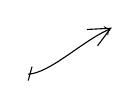
\begin{tikzpicture}[scale=.8]
\draw[->] (0,0) .. controls (.35,.02) and (.85,.52) .. (1.3,.72);
\draw (0,-.10)--(.06,.12);
\draw (.93,.71)--(1.31,.73)--(1.10,.45);
\end{tikzpicture}}

% E537-04
alors les hom induits par $\delta_G$
% E537-05
\[
(33)\qquad
\diagram{\begin{tikzcd}[ampersand replacement=\&,column sep=large]
Z_\rho\arrow[r,"{\delta_\rho}"]\&\gamma_{\rho,\sigma}
\end{tikzcd}},
\qquad
\diagram{\begin{tikzcd}[ampersand replacement=\&,column sep=large]
Z_\sigma\arrow[r,"{\delta_\sigma}"]\&\gamma_{\rho,\sigma}
\end{tikzcd}}
\]
% E537-06
ont
% E537-07
\deleted{comme}
% E537-08
\inserted{des}
images qui contiennent $\gamma'_{\rho,\sigma}$ et
$\gamma''_{\rho,\sigma}$ respectivement,
% E537-09
\deleted{et \unsure{sss|ssi} \unsure{à}}

% E537-10
\deleted{D'ailleurs l'image de $Z_\rho$ est contenue dans
$\gamma'_{\rho,\sigma}$
% E537-11
\deleted{si on suppose}
% E537-12
\inserted{(\unsure{ou égale}) \unsure{sss|ssi}}
$\rho$ et $\rho^{-1}$ non conjugués dans $\mathcal{G}$,
% E537-13
\deleted{il suffit}
% E537-14
\inserted{et de}
% E537-15
\deleted{\unsure{pour ceci}}
$\overline{\mathrm m}$ l'image de $Z_\sigma$ est
\unsure{réduite|réduit} à $\gamma''_{\rho,\sigma}$
\unsure{sss|ssi} $\sigma$ et $\sigma^{-1}=-\sigma$
non conjugués dans $\mathcal{G}$. Notons p.ex.
% E537-16
\deleted{que}
% E537-17
\inserted{si}
% E537-18
\deleted{$\mathcal{G}=\mathrm{SL}(2,\widehat{\mathbb{Z}})'$,}
$\sigma^2=1$,
\unsure{la} dernière condition n'est pas \unsure{satisfaite},
donc
% E537-19
$\diagram{\begin{tikzcd}[ampersand replacement=\&]
Z_\sigma\arrow[r]\&\gamma_{\rho,\sigma}
\end{tikzcd}}$
est surjective,
% E537-20
\deleted{elle ne}
% E537-21
\inserted{\deleted{\unsure{mais}} elle}
l'est
% E537-22
\deleted{pas non plus}
% E537-23
\deleted{\unsure{qu'elle est satisfaite si}}
$\mathcal{G}=\unsure{\mathrm{SL}}(2,\widehat{\mathbb{Z}})$
% E537-24
\inserted{dans $\mathrm{SL}(2,\widehat{\mathbb{Z}})$}
$\sigma$ y est conjugué à $-\sigma$, par le
% E537-25
\deleted{(car $\sigma$ et}
\unsure{th.} général de Steinberg p.ex.) ---
\unsure{se peut-il produire} dans le \unsure{cas}
universel $\mathrm{SL}(2,\mathbb{Z})^{\wedge}
=\mathcal{G}_{1,1}^{+\wedge}$?
}

% E537-26
\margin{\deleted{
La condition sur $\rho$ est non satisfaite
% E537-27
\deleted{\unsure{pour}}
$\mathcal{G}=\mathrm{SL}(2,\widehat{\mathbb{Z}})/\pm1$,
Comme dans ce cas les \uline{deux} hom
% E537-28
$\diagram{\begin{tikzcd}[ampersand replacement=\&,column sep=small]
Z_\rho,\deleted{\unsure{Z_\sigma}}\arrow[r]\&
\unsure{\widehat{\gamma}_{\rho,\sigma}|\gamma_{\rho,\sigma}}
=\widehat{\mathbb{Z}}^{*}
\end{tikzcd}}$,
% E537-29
$\diagram{\begin{tikzcd}[ampersand replacement=\&,column sep=small]
Z_\sigma\arrow[r]\&\gamma_{\rho,\sigma}=\widehat{\mathbb{Z}}^{*}
\end{tikzcd}}$
sont \unsure{surjections|surjectives}),
mais elle l'est pour $\mathcal{G}=\mathrm{SL}(2,\widehat{\mathbb{Z}})$,
car on trouve que l'image de
% E537-30
$\diagram{\begin{tikzcd}[ampersand replacement=\&,column sep=small]
\unsure{Z_\rho}\arrow[r]\&\gamma_{\rho,\sigma}
\end{tikzcd}}$
est $\gamma'_{\rho,\sigma}$.
Mais dans $\unsure{\mathcal{G}_{0,3}^{+\wedge}}$,
$\rho$ et $\rho^{-1}$ sont aussi non conjugués,
i.e. l'image est \unsure{réduite} aussi à $\gamma'_{\rho,\sigma}$.
}}
% E537-31
\margin{536}

% E537-F01
\margin{\begin{center}
536\\
\texttt{https://grothendieck.umontpellier.fr}\\
Université de Montpellier, UMR CNRS 5149, Case courrier 051, Place Eugène Bataillon\\
34095 Montpellier cedex 5 - France
\end{center}}

\scanpage{538}
% E538-01
\mspage{572}

% E538-02
\uline{Proposition} \quad 1°) L'image $\delta_\rho(Z_\rho)$ contient
$\gamma'_{\rho,\sigma}$, et est
% E538-03
\deleted{\unsure{ég}}
% E538-04
réduite à $\gamma'_{\rho,\sigma}$ \unsure{sss|ssi}
$\rho$ et $\rho^{-1}$ non conjugués dans $\mathcal{G}$ ---
donc elle est égale à $\gamma_{\rho,\sigma}$
i.e.
% E538-05
$\delta_\rho:\diagram{\begin{tikzcd}[ampersand replacement=\&,column sep=large]
Z_\rho\arrow[r]\&\gamma_{\rho,\sigma}
\end{tikzcd}}$
% E538-06
épi \unsure{sss|ssi} $\rho$ et $\rho^{-1}$ sont conjugués dans $\mathcal{G}$.

% E538-07
2°) L'image $\delta_\sigma(Z_\sigma)$ contient
$\gamma''_{\rho,\sigma}$, et elle est réduite à
$\gamma''_{\rho,\sigma}$ \unsure{sss|ssi} $\sigma$ et
$\sigma^{-1}=-\sigma$ non conjugués dans $\mathcal{G}$ ---
\unsure{donc|sinon} elle est égale à $\gamma_{\rho,\sigma}$ i.e.
% E538-08
$\delta_\sigma:\diagram{\begin{tikzcd}[ampersand replacement=\&,column sep=large]
Z_\sigma\arrow[r]\&\gamma_{\rho,\sigma}
\end{tikzcd}}$
% E538-09
épi \unsure{sss|ssi} $\sigma$ et
$\unsure{-\sigma^{-1}|\sigma^{-1}}=-\sigma$ sont conjugués dans $\mathcal{G}$.

% E538-10
\uline{Corollaire 1}. Si $\mathcal{G}$ contient comme quotient
% E538-11
\[
SL(2,\mathbb{Z}/3\mathbb{Z})',\quad\text{avec}\quad
\rho=\begin{pmatrix}0&1\\-1&1\end{pmatrix},\qquad
\sigma=\begin{pmatrix}0&-1\\1&0\end{pmatrix}
\]
% E538-12
$(\bmod\ \pm1)$, alors l'image de $\delta_\rho$ est
$\gamma'_{\rho,\sigma}$.

% E538-13
En effet, on voit que $\rho$ et $\pm\rho^{-1}$ ne sont
conjugués dans $\mathcal{G}$, car ils ne le sont
pas dans $SL(2,\mathbb{Z}/3\mathbb{Z})'$ ---
% E538-14
\deleted{\unsure{par ex.}\ \unsure{pour}}
% E538-15
\inserted{Vérifions le:}
% E538-16
$\rho$ et $-\rho^{-1}$ ont déjà des traces distinctes
$1$ et $-1$, $\unsure{\in}(\mathbb{Z}/3\mathbb{Z})^{\unsure{*}}$,
ils ne sont pas conjugués.

% E538-17
On a
% E538-18
\[
(\underbrace{\tau\sigma}_{\tau'_\infty})(\rho)=\rho^{-1},
\]
% E538-19
donc
% E538-26
\deleted{tous} les éléments de
% E538-20
\deleted{$f\in$}
% E538-21
$GL(2,\mathbb{Z}/3\mathbb{Z})$
% E538-22
\deleted{tels que}
% E538-23
qui conjuguent $\rho$ en $\rho^{-1}$ sont de la forme
$f\tau'_\infty$, où
% E538-24
$f=\unsure{c|b}\rho+d$, on \unsure{veut}
$\det(f\tau'_\infty)=1$ i.e. $\det(f)=-1$
$(\text{car }\det(\tau'_\infty)=-1)$,
i.e. $c^2+\unsure{cd}+d^2=-1$, impossible.
% E538-25
\margin{537}

% E538-F01
\margin{\begin{center}
537\\
\texttt{https://grothendieck.umontpellier.fr}\\
Université de Montpellier, UMR CNRS 5149, Case courrier 051, Place Eugène Bataillon\\
34095 Montpellier cedex 5 - France
\end{center}}

\scanpage{539}

% E539-01
\uline{Corollaire 2}\quad Si $\sigma^2=1$, alors
% E539-02
$\diagram{\begin{tikzcd}[ampersand replacement=\&,column sep=large]
Z_\sigma\arrow[r]\&\gamma_{\rho,\sigma}
\end{tikzcd}}$
% E539-03
est surjectif. Si Par contre $\mathcal{G}$ contient comme quotient
% E539-04
\deleted{$\mathbb{Z}/4\mathbb{Z}$}
% E539-05
$SL(2,\mathbb{Z}/4\mathbb{Z})$
$(\uline{\text{sans}}\ \prime\ !)$, avec $\rho,\sigma$ comme
\unsure{d'habitude}, alors
% E539-06
\[
\operatorname{Im}(\delta_\sigma)=\gamma''_{\rho,\sigma}.
\]

% E539-07
Il faut voir que $\sigma$ et $\sigma^{-1}=-\sigma$ non conjugués
dans $SL(2,\mathbb{Z}/4\mathbb{Z})$, en utilisant que
$\tau_\infty(\sigma)=\sigma^{-1}$, donc
% E539-08
\deleted{il f}
% E539-09
les \unsure{élts|élms} de $GL(2,\mathbb{Z}/4\mathbb{Z})$ qui
conjuguent $\sigma$ en $\sigma^{-1}$ sont les
% E539-10
\inserted{$g=f\tau_\infty$ avec}
% E539-11
$f=t\sigma+\unsure{u|n}$,
% E539-12
\deleted{\unsure{avec}}
% E539-13
et donc que $\det(g)=1$ signifie $\det f=-1$
i.e. $t^2+\unsure{u|n}^2=-1$, impossible.

% E539-14
\deleted{
Posons
% E539-15
\[
(34)\qquad
\left\{
\begin{aligned}
SZ_\rho&=
% E539-16
\inserted{\operatorname{Ker}\delta_\rho=}
Z_\rho\cap\mathcal{G}=\operatorname{Centr}_{\mathcal{G}}(\rho).\\
SZ_\sigma&=
% E539-17
\inserted{\operatorname{Ker}\delta_\sigma=}
Z_\sigma\cap\mathcal{G}=\operatorname{Centr}_{\mathcal{G}}(\sigma)\\
SB_{\rho,\sigma}&=\operatorname{Ker}\delta_B
=B_{\rho,\sigma}\cap\mathcal{G}=L_0.
\end{aligned}
\right.
\]
}

% E539-18
\deleted{
% E539-19
\[
(35)\qquad
\begin{aligned}
&S_0\unsure{\mathcal{M}|M}_{\rho,\sigma}
\subset B_{\rho,\sigma}\times\unsure{Z_\rho|N_\rho}
\times Z_\sigma\times\unsure{G_{\rho,\sigma}|\gamma_{\rho,\sigma}}\\
&\text{''}\\
&\bigl\{(u,a,b,U\unsure{\}|)}\ \bigm|\,
\delta_B(u)=\delta_G(U)=\delta_\sigma(b)
=\varepsilon_3(\mu)\delta_\rho(a)\bigr\}
\end{aligned}
\]
}
% E539-20
\margin{538}

% E539-F01
\margin{\begin{center}
538\\
\texttt{https://grothendieck.umontpellier.fr}\\
Université de Montpellier, UMR CNRS 5149, Case courrier 051, Place Eugène Bataillon\\
34095 Montpellier cedex 5 - France
\end{center}}

\scanpage{540}
% E540-01
\mspage{573}

% E540-02
% E540-03
Notons que d'après (2), \inserted{(4)}, on a
% E540-04
\[
(35)\qquad \tau_B \overset{\mathrm{dfn}}{=}(\tau,-1)\in B_{\rho,\sigma}
\]
% E540-05
Et évidemment $\tau_B\notin L_0=B_{\rho,\sigma}\cap\mathcal{G}$.
Donc on a un plongement
% E540-06
\[
(36)\qquad
\left\{
\begin{array}{l}
\diagram{\begin{tikzcd}[ampersand replacement=\&,column sep=large,row sep=small]
\mathcal{G}'=\{1,\tau\}.\mathcal{G} \arrow[r,hook] \& G_{\rho,\sigma}\\
\tau \arrow[r,mapsto] \& \tau_B\\
g \arrow[r,mapsto] \& g\quad\text{si }g\in\mathcal{G}
\end{tikzcd}}
\end{array}
\right.,
\]
% E540-07
\margin{\uline{NB} $\mathcal{G}'$ est un quotient de
$\mathrm{GL}(2,\mathbf{Z})^\wedge$, et $\tau$ y correspond à
l'image de l'élément
$\tau_\infty=\begin{pmatrix}-1&0\\0&1\end{pmatrix}$
de $\unsure{\mathrm{GL}(2,\mathbf{Z})}$.}

% E540-08
% E540-09
donc l'\unsure{autom} $\tau$ de $\mathcal{G}$ sera considéré comme
induit par \deleted{\unsure{l'élé}} $\operatorname{int}(\tau_B)$,
où $\tau_B$ est considéré lui-$\overline{\mathrm m}$ comme un
élément de $G_{\rho,\sigma}$.

% E540-10
% E540-11
\deleted{\illegible{2}} En relation avec l'égalité
% E540-12
\[
\tau_B(\sigma)=\sigma^{-1}\quad(=-\sigma)
\]
% E540-13
% E540-14
% E540-15
% E540-16
% E540-18
% E540-17
qui montre que $\tau_B$ normalise le sous-groupe
\inserted{$L_\sigma$} \inserted{engendré par $\sigma$}
(isomorphe à un quotient de $\mathbf{Z}/4\mathbf{Z}$),
\deleted{\unsure{groupe}} \inserted{donc}
\inserted{normalise $Z_\sigma=\operatorname{Centr}_{G_{\rho,\sigma}}(L_\sigma)$},
\deleted{\unsure{puis introduisons}} introduisons
% E540-19
\[
(37)\qquad
N_\sigma=\underset{(\text{$1/2$ direct})}{\{1,\tau_B\}.Z_\sigma},
\]
% E540-20
et l'hom. canonique
% E540-21
\[
(38)\qquad
\left\{
\begin{array}{l}
\diagram{\begin{tikzcd}[ampersand replacement=\&,column sep=large,row sep=small]
N_\sigma \arrow[r,"i_\sigma"] \& G_{\rho,\sigma} \& \&\\
\tau_B \arrow[r,mapsto] \& \tau_B, \& x \arrow[r,mapsto] \& x\quad\text{si }x\in Z_\sigma
\end{tikzcd}}
\end{array}
\right..
\]

% E540-22
\deleted{Cet hom. est injectif sss}
% E540-23
% E540-24
L'image de cet hom. n'est autre que le normalisateur de $\sigma$
dans $G_{\rho,\sigma}$, car un \deleted{\unsure{autom}}
$g\in G_{\rho,\sigma}$ qui normalise $L_\sigma$ doit transformer
$\sigma$ en un générateur de $L_\sigma$, i.e. en $\sigma$ ou
$\sigma^{-1}$, dans le premier cas on aura $g\in Z_\sigma$, dans
le deuxième $g(\sigma)=\tau_B(\sigma)$ i.e. $\tau_B^{-1}g\in Z_\sigma$
i.e. $g\in\tau_B Z_\sigma$. L'hom (38) est injectif

% E540-25
\margin{539}

% E540-F01
\margin{\begin{center}
539\\
\texttt{https://grothendieck.umontpellier.fr}\\
Université de Montpellier, UMR CNRS 5149, Case courrier 051, Place Eugène Bataillon\\
34095 Montpellier cedex 5 - France
\end{center}}

\scanpage{541}
% E541-01
\deleted{sss $\tau_B\in Z$}
% E541-02
sss $\tau_B\notin Z_\sigma$ i.e. $\sigma\ne\sigma^{-1}$ i.e.
$\sigma^2\ne1$ i.e. "$-1$" $\ne1$.

% E541-03
Puisqu'on y est, profitons de la formule
% E541-04
\[
\tau_B(\rho)=\sigma(\rho^{-1})
\]
% E541-05
pour introduire
% E541-06
\[
(39)\qquad
\tau'\uuline{=}\sigma^{-1}\tau\in\mathcal{G}'\subset G_{\rho,\sigma}
\]
% E541-07
(qui correspond à l'élément
% E541-08
% E541-09
\[
(40)\qquad
\tau'_\infty=\sigma_\infty^{-1}\tau_\infty
=-\sigma_\infty\tau_\infty
=\begin{pmatrix}0&1\\1&0\end{pmatrix}
\in\underbrace{\mathrm{GL}(2,\mathbf{Z})}_{
\inserted{\substack{\Vert\\\mathcal{T}_{1,1}}}}
\biggr),
\]

% E541-10
% E541-11
\deleted{\unsure{qui est}} on aura donc
% E541-12
\[
(40)\qquad \tau'^2=1,\qquad \tau'(\rho)=\rho^{-1}.
\]

% E541-13 deletion
\deleted{Introduisons donc}
% E541-14 deletion
\deleted{$(41)\qquad N_\rho=\{1,\tau'\}.$}
% E541-15
% E541-16
\inserted{Ainsi $\tau'$ normalise le sous-groupe $L_\rho$
(isomorphe à un quotient de $\mathbf{Z}/6\mathbf{Z}$) engendré
par $\rho$, donc il normalise le centralisateur
\inserted{$Z_\rho$} de $L_\rho$, et on peut construire}
% E541-17
% E541-18
\margin{\uline{NB} On a en $\overline{\mathrm m}$ temps
$\tau'(\sigma)=\sigma^{-1}$, donc on peut considérer $\tau'$
comme élément de $N_\sigma$, et \deleted{\illegible{1}} on a
$N_\sigma=\{1,\tau'\}.Z_\sigma$ (qui est $1/2$ direct)}
% E541-19
\[
(41)\qquad
N_\rho\overset{\mathrm{dfn}}{=}
\underset{(\text{semi-direct})}{\{1,\tau'\}.Z_\rho}
\]
% E541-20
% E541-21
% E541-22
et \deleted{\unsure{un}} \deleted{\unsure{du}} hom. canonique
% E541-23
\[
(42)\qquad
\left\{
\begin{array}{l}
\diagram{\begin{tikzcd}[ampersand replacement=\&,column sep=large,row sep=small]
N_\rho \arrow[r,"i_\rho"] \& G_{\rho,\sigma} \& \&\\
\tau' \arrow[r,mapsto] \& \tau', \& x \arrow[r,mapsto] \& x\quad\text{pour }x\in Z_\rho
\end{tikzcd}}
\end{array}
\right..
\]

% E541-24
% E541-25
% E541-26
% E541-27
L'image de cet hom. est le normalisateur de $L_\rho$ dans
$G_{\rho,\sigma}$ --- on le voit comme \unsure{t-à-l} pour $i_\sigma$,
en notant que \deleted{les}
\inserted{$\rho,\rho^{-1}$ sont les \uline{seuls}} générateurs de
$L_\rho$. L'hom $i_\rho$ est injectif sss $\tau'\notin Z_\rho$
i.e. \deleted{\unsure{sss}} $\rho\ne\rho^{-1}$ i.e. $\rho^2\ne1$
i.e. $\rho\ne-1$
% E541-28
% E541-29
% E541-30
% E541-31
% E541-32
(\deleted{\unsure{en ce cas}}
\inserted{NB \uline{$\rho=-1$}}
\deleted{\unsure{implique}} \deleted{\unsure{équivalent}}
\deleted{\unsure{en fait}} que $\rho$ commute à $\sigma$, et que
$\mathcal{G}$ est un quotient de $\mathbf{Z}/12\mathbf{Z}$, avec
$\rho$ correspondant à $2$
% E541-33 insertion
\inserted{et $\sigma$ à $3$, mais ici $2\rho=0$ donc
$\mathcal{G}$ est un quotient de $\mathbf{Z}/4\mathbf{Z}$ avec
$\rho$ correspondant à $2$, $\sigma$ à $3=-1\ldots$}).

% E541-34
% E541-35
\margin{
\[
(43)\qquad\left\{
\begin{array}{l}
\diagram{\begin{tikzcd}[ampersand replacement=\&,column sep=huge,row sep=large]
N_\rho \arrow[r,"\delta_\rho=\delta_G\circ i_\rho"] \& \gamma_{\rho,\sigma}\\
N_\sigma \arrow[r,"\delta_\sigma=\delta_G\circ i_\sigma"] \& \gamma_{\rho,\sigma}
\end{tikzcd}}\\
\hfill\text{épimorphismes}
\end{array}
\right.
\]}
% E541-36
\margin{"On a fait ce qu'il fallait" pour avoir des
\uline{épimorph.} $\unsure{\varphi}$.}
% E541-37
\margin{540}

% E541-F01
\margin{\begin{center}
540\\
\texttt{https://grothendieck.umontpellier.fr}\\
Université de Montpellier, UMR CNRS 5149, Case courrier 051, Place Eugène Bataillon\\
34095 Montpellier cedex 5 - France
\end{center}}

\scanpage{542}
\mspage{574}
% E542-01
\deleted{\(\unsure{(43)}\)}
% E542-02
\unsure{Situons|Soit}
% E542-03
\deleted{\(\unsure{\mathfrak{g}|g}\)}

% E542-04
\[
(44)\qquad
\begin{gathered}
S\unsure{\mathfrak{g}|g}_{\rho,\sigma}^{\unsure{*}}
\subset \mathcal{G}'\times\mathcal{G}\times\widehat{\mathbb Z}^{*}
\\[-2pt]
\Vert\\[-2pt]
\left\{(\alpha,\beta,\mu)\ \left|
\begin{array}{l}
\alpha\equiv\tau^{\nu_3(\mu)}\bmod\mathcal{G}
\quad\text{i.e. }\chi(\alpha)=\varepsilon_3(\mu)\\
\underbrace{\alpha\rho(\alpha)^{-1}}_{\zeta}
=\underbrace{\varepsilon_2(\mu)\beta\sigma(\beta)^{-1}}_{\eta}
\ell_1^\nu,\quad\text{où}
\end{array}\right.\right\}
\end{gathered}
\]
% E542-05
\inserted{\[
\nu=(\mu-1)/2,\qquad\uline{(\ell_1=\varepsilon_1^2)}
\]}

% E542-06
\deleted{\[
(\unsure{36})\qquad
\unsure{\mathfrak{g}|g}_{\rho,\sigma}^{\unsure{*}\,\mathrm{eff}}
=\left\{(\alpha,\beta,\mu)\in
\unsure{\mathfrak{g}|g}_{\rho,\sigma}^{*}\ \middle|\ \unsure{\exists}\right.
\]}

% E542-07
d'où

% E542-08
% E542-09
\begin{samepage}
\[
(45)
\]
\diagram{\(
\left\{
\begin{gathered}
\begin{tikzcd}[ampersand replacement=\&,column sep=large]
S\unsure{\mathfrak{g}|g}_{\rho,\sigma}^{\unsure{*}}
\arrow[r] \&
\begin{gathered}
\Sigma_{\rho,\sigma}\subset\mathcal{G}\times\mathcal{G}\times\widehat{\mathbb Z}^{*}\\[-2pt]
\Vert\quad\mathrm{dfn}\\[-2pt]
\left\{(\zeta,\eta,\mu)\ \left|
\begin{array}{l}
\zeta\rho\ \text{conj. ds }\mathcal{G}:\rho^\mu\\
\unsure{\eta|\zeta}\sigma\quad\underline{\hspace{7em}}\quad\sigma^\mu\\
\zeta=\deleted{\unsure{\beta\sigma(\beta)^{-1}}}\eta\ell_1^\nu
\end{array}\right.\right.
\end{gathered}\\
(\alpha,\beta,\mu)\arrow[r,mapsto]\&
\left(\overbrace{\alpha\rho(\alpha)^{-1}}^{[\alpha,\rho]},
\varepsilon_2(\mu)\overbrace{\beta\sigma(\beta)^{-1}}^{[\beta,\sigma]},\mu\right).
\end{tikzcd}
\end{gathered}
\right.
\)}
\end{samepage}
% E542-10
\inserted{\((\text{où }\nu=(\mu-1)/2\)}
% E542-11
On désigne par
\(\unsure{\mathfrak{g}|g}_{\rho,\sigma}^{\unsure{*}\,\mathrm{eff}}\)
l'image inverse de
\(\Sigma_{\rho,\sigma}^{\mathrm{eff}}\)
(cf cor. p. 570). \(\simeq B_{\rho,\sigma}\).
Par \unsure{construction}
% E542-12
\inserted{on trouve donc une application \uline{surjective}}
% E542-13
\margin{
\((\unsure{46\mathrm{bis}})\)
\diagram{\begin{tikzcd}[ampersand replacement=\&]
S\unsure{\mathfrak{g}|g}_{\rho,\sigma}^{\mathrm{eff}}
\arrow[r,"\text{épi.}"]\&[30pt]
\Sigma_{\rho,\sigma}^{\mathrm{eff}}
\end{tikzcd}}
}

% E542-14
On considère
\(S\unsure{\mathfrak{g}|g}_{\rho,\sigma}^{*}\)
comme contenu dans un
% E542-15
\deleted{groupe}
% E542-16
\inserted{ens.}
% E542-17
plus gros

% E542-18
% E542-19
\[
(47)\qquad
\begin{gathered}
\unsure{\mathfrak{g}|g}_{\rho,\sigma}^{\unsure{*}}
\subset G_{\rho,\sigma}\times G_{\rho,\sigma}
\times\widehat{\mathbb Z}^{*}
\\[-2pt]
\Vert\\[-2pt]
\left\{(\alpha,\beta,\mu)\ \left|
\begin{array}{l}
\chi(\alpha)\equiv\varepsilon_3
\bigl(\deleted{\unsure{\chi(\mu)|\chi(\beta)}}\mu\bigr)
\chi(\beta);\\
\underbrace{\alpha\rho(\alpha)^{-1}}_{=\alpha(\rho)\rho^{-1}=\zeta}
=
\underbrace{\varepsilon_2(\mu)\beta\sigma(\beta)^{-1}}_
{=\varepsilon_2(\mu)\beta(\sigma)\sigma^{-1}=\eta}
\ell_1^\nu
\end{array}\right.\right\}
\end{gathered}
\]
% E542-20
de sorte que l'on aura
% E542-21
% E542-22
\[
(48)\qquad
\begin{aligned}
S\unsure{\mathfrak{g}|g}_{\rho,\sigma}^{\unsure{*}}
&=\unsure{\mathfrak{g}|g}_{\rho,\sigma}^{\unsure{*}}
\cap\bigl(\mathcal{G}'\times\mathcal{G}\times\widehat{\mathbb Z}^{*}\bigr),
\\
&=\left\{(\alpha,\beta,\mu)\in
\unsure{S\mathfrak{g}|Sg}_{\rho,\sigma}^{*}
\ \left|
\begin{array}{l}
\delta_\sigma(\beta)=1\deleted{\unsure{\}}}\\
\delta_\rho\bigl(\alpha\tau^{\nu_3(\mu)}\bigr)=1
\end{array}\right.\right\}
\end{aligned}
\]
% E542-23
\margin{541}

% E542-F01
\margin{\begin{center}
541\\
\texttt{https://grothendieck.umontpellier.fr}\\
Université de Montpellier, UMR CNRS 5149, Case courrier 051, Place Eugène Bataillon\\
34095 Montpellier cedex 5 - France
\end{center}}

\scanpage{543}
% E543-01
et on a encore une application canonique
% E543-02
\begin{samepage}
\[
(49)
\]
\diagram{\(
\left\{
\begin{gathered}
\begin{tikzcd}[ampersand replacement=\&,column sep=large]
\unsure{\mathfrak{g}|g}_{\rho,\sigma}^{*}\arrow[r]\&
\Sigma_{\rho,\sigma}^{\unsure{*}}\\
(\alpha,\beta,\mu)\arrow[r,mapsto]\&
\bigl([\alpha,\rho],\varepsilon_2(\mu)[\beta,\sigma],\mu\bigr).
\end{tikzcd}
\end{gathered}
\right.
\)}
\end{samepage}

% E543-03
\deleted{\unsure{dont l'i}}
% E543-04
On note
\(\unsure{\mathfrak{g}|g}_{\rho,\sigma}^{\mathrm{eff}}\)
l'image inverse de
\(\Sigma_{\rho,\sigma}^{\mathrm{eff}}\),
et on trouve
% E543-05
\[
(50)\qquad
\begin{aligned}
S\unsure{\mathfrak{g}|g}_{\rho,\sigma}^{\mathrm{eff}}
&=\unsure{\mathfrak{g}|g}_{\rho,\sigma}^{\mathrm{eff}}
\cap\bigl(\mathcal{G}'\times\mathcal{G}\times\widehat{\mathbb Z}^{*}\bigr)
\\
&=\left\{(\alpha,\beta,\mu)\in
\unsure{\mathfrak{g}|g}_{\rho,\sigma}^{\mathrm{eff}}
\ \left|
\begin{array}{l}
\delta_\sigma(\beta)=1\\
\unsure{\delta_\rho|\delta_B}\bigl(\alpha{\tau'}^{\nu_3(\mu)}\bigr)=1
\end{array}\right.\right\}
\end{aligned}
\]

% E543-06
On a une section de
% E543-07
% E543-08
% E543-09
% E543-10
\begin{samepage}
\[
(51)
\]
\diagram{
\begin{tikzcd}[ampersand replacement=\&,column sep=large,row sep=large]
\unsure{\mathfrak{g}|g}_{\rho,\sigma}^{\mathrm{eff}}\arrow[r]\&
\Sigma_{\rho,\sigma}^{\mathrm{eff}}\&
\zeta=[u,\rho],\overset{\inserted{\eta=}}{[u,\sigma]},
\overset{\inserted{\mu=}}{\chi_B(u)}
\\
\& B_{\rho,\sigma}
\arrow[u,"\sim"']
\arrow[ul,"\text{\uline{section}}"]\&
u\deleted{\unsure{\varphi|*}}\arrow[u,mapsto]
\end{tikzcd}
}
\end{samepage}

% E543-11
donnée par
% E543-12
% E543-13
% E543-14
\begin{samepage}
\[
(52)
\]
\diagram{\begin{tikzcd}[ampersand replacement=\&,column sep=large]
u\deleted{\unsure{\varphi|*}}\arrow[r,mapsto]\&
\bigl(\deleted{\unsure{\alpha=}}u,\,
u{\tau'}^{\nu_2(\mu)},\,\mu=\chi_B(u)\bigr)
\end{tikzcd}}
\end{samepage}

% E543-15
puisqu'on aura
(posant \(\varepsilon=\varepsilon_2(\mu)
\unsure{\overset{\mathrm{dfn}}{=}|=}
(-1)^{\nu_2}\).)
% E543-16
\[
[u,\rho]=u\rho(u)^{-1}=\zeta
\]
% E543-17
\[
\begin{aligned}
\varepsilon
\left[u{\tau'}^{\nu_2(\mu)=\nu_2},\sigma\right]
&=\varepsilon u{\tau'}^{\nu_2}
\sigma\bigl(u\unsure{\tau|\tau'}^{\nu_2}\bigr)^{-1}\\
&=\varepsilon u
\left(\underbrace{
\unsure{\tau|\tau'}^{\nu_2}
\sigma\bigl(\unsure{\tau|\tau'}^{\nu_2}\bigr)^{-1}
}_{=\varepsilon}\right)\sigma(u)^{-1}
=\unsure{\varepsilon u|u}\sigma(u)^{-1}=\eta
\end{aligned}
\]
% E543-18
OK. Donc
% E543-19
\deleted{\unsure{l'ens|les}}
% E543-20
% E543-21
\inserted{l'ens \deleted{\unsure{des}}
\(\unsure{\mathfrak{g}_{\rho,\sigma}(u,\mu)|g_{\rho,\sigma}^{(u,\mu)}}\)}
% E543-27
des \((\alpha,\beta,\mu)\,\unsure{-}\)
donnant \unsure{l'image}
% E543-22
% E543-23
% E543-24
\[
(\zeta,\eta,\mu)\deleted{\unsure{\Longrightarrow|=}}
\unsure{[|(}\,[u,\rho],[u,\sigma],
\overset{\inserted{\mu=}}{\chi_B(u)}\bigr)
\]
% E543-25
\unsure{sera exactement}
% E543-26
\margin{542}

% E543-F01
\margin{\begin{center}
542\\
\texttt{https://grothendieck.umontpellier.fr}\\
Université de Montpellier, UMR CNRS 5149, Case courrier 051, Place Eugène Bataillon\\
34095 Montpellier cedex 5 - France
\end{center}}

\scanpage{544}
\mspage{575}
% E544-01
\deleted{\unsure{les}}
% E544-02
\inserted{\(
\unsure{\mathfrak{g}_{\rho,\sigma}(u,\mu)|g_{\rho,\sigma}^{(u,\mu)}}
=
\)}
% E544-03
\[
(53)\qquad
\left\{\left(
\overbrace{ua_0^{-1}}^{\alpha},
\overbrace{u{\tau'}^{\nu_2}b_0^{-1}}^{\unsure{\beta|b}},
\mu\right)
\ \middle|\ a_0\in Z_\rho,\ b_0\in Z_\sigma,\
\nu_2=\nu_2(\mu)\right\}
\]
% E544-04
\inserted{\[
\bigl(=(ua_0^{-1},ub^{-1},\mu)\unsure{\}}
\quad\text{où}\quad b=b_0{\tau'}^{\unsure{\nu_2}}
\]}
% E544-05
qu'on écrit aussi
% E544-06
% E544-29
\[
(54)\qquad
\unsure{\mathfrak{g}_{\rho,\sigma}(u,\mu)|g_{\rho,\sigma}^{(u,\mu)}}
=
\left\{\left(
\underbrace{ua_0^{-1}}_{\alpha},
\underbrace{u\,i_\sigma(b)}_{\beta},
\mu\right)
\ \middle|\ 
a_0\in Z_\rho,\ 
\underset{\inserted{\text{(cf (37)(38))}}}{b\in N_\sigma},\
\boxed{\varepsilon_\sigma(b)=\varepsilon_2(\mu)}
\right\}
\]
% E544-07
où \(\varepsilon_\sigma:N_\sigma\longrightarrow\{\pm1\}\)
est défini sur (37) comme l'hom. can.
s'insérant dans la suite exacte
% E544-08
\begin{samepage}
\[
(55)
\]
\diagram{\begin{tikzcd}[ampersand replacement=\&]
1\arrow[r]\&Z_\sigma\arrow[r]\&N_\sigma
\arrow[r,"\varepsilon_\sigma"]\&
\underbrace{\{\pm1\}}_{\simeq\{1,\tau'\}}\arrow[r]\&1.
\end{tikzcd}}
\end{samepage}

% E544-09
Si on cherche l'ens des éléments de
\(S\unsure{\mathfrak{g}|g}_{\rho,\sigma}^{\mathrm{eff}}\)
au dessus de \((\zeta,\eta,\mu)\), il faut de plus
imposer les conditions
% E544-10
\[
(56)\qquad
\deleted{\unsure{\alpha=}}ua_0^{-1}{\tau'}^{\nu_3(\mu)}\in\mathcal{G},
\quad u\,i_\sigma(b)\in\mathcal{G}
\]
% E544-11
i.e.
\[
\delta_G(ua_0^{-1}{\tau'}^{\nu_3})=1,\quad
\delta_G(u\,i_\sigma(b))=1
\]
% E544-12
soit encore
% E544-13
\[
(57)\qquad
\delta_G(u)=
\underbrace{\delta_\sigma(b)}_{\text{cf (43)}}
=
\underbrace{\delta_\rho}_{\text{cf (43)}}
({\tau'}^{\nu_3}.a_0).
\]
% E544-14
Posons donc
\[
a={\tau'}^{\nu_3}.a_0\quad\text{\unsure{ds|dans}}\ N_\rho
\]
% E544-15
\inserted{\((\text{donc }a_0={\tau'}^{\nu_3}a)\)}
% E544-16
on voit que
% E544-17
\[
(54)\qquad
\unsure{\mathfrak{g}_{\rho,\sigma}(u,\mu)|g_{\rho,\sigma}^{(u,\mu)}}
=
\left\{(ua^{-1}{\tau'}^{\nu_3},ub^{-1},\mu)\ \left|
\begin{array}{l}
a\in N_\rho,\ b\in N_\sigma\ \text{tels que}\\
\varepsilon_\rho(a)=\varepsilon_3(\mu),\
\varepsilon_\sigma(b)=\varepsilon_2(\mu)\\
\delta_\rho(a)=\delta_\sigma(b)=\delta_G(u)
\end{array}\right.\right\}
\]

% E544-18
Introduisons donc le groupe
% E544-19
% E544-20
\[
(55)\qquad
\deleted{\unsure{S_0}}
\unsure{\mathcal{M}|M}_{\rho,\sigma}[0]
=\unsure{B}_{\rho,\sigma}
\times_{\gamma_{\rho,\sigma}}N_\rho
\times_{\gamma_{\rho,\sigma}}N_\sigma.
\]
% E544-21
et les homomorphismes composés
% E544-22
% E544-23
% E544-24
\begin{samepage}
\[
(56)
\]
\diagram{\(
\left\{
\begin{gathered}
\begin{tikzcd}[ampersand replacement=\&,column sep=large]
\deleted{\unsure{S_0}}\unsure{\mathcal{M}|M}_{\rho,\sigma}[0]
\arrow[r]\&N_\rho\&
\overset{\varepsilon_\rho}{\unsure{\longleftrightarrow|\longrightarrow}}\&
\{\pm1\}
\\
\deleted{\unsure{S_0}}\unsure{\mathcal{M}|M}_{\rho,\sigma}[0]
\arrow[r]\&N_\sigma\arrow[rr,"\varepsilon_\sigma"]\&\&
\{\pm1\}
\end{tikzcd}
\end{gathered}
\right.
\)}
\end{samepage}
% E544-25
% E544-28
\margin{\deleted{\unsure{notés}\ \(\varepsilon'_\rho\)}}
% E544-26
(encore notés \(\varepsilon_\rho,\varepsilon_\sigma\)
par abus de notation)
% E544-27
\margin{543}

% E544-F01
\margin{\begin{center}
543\\
\texttt{https://grothendieck.umontpellier.fr}\\
Université de Montpellier, UMR CNRS 5149, Case courrier 051, Place Eugène Bataillon\\
34095 Montpellier cedex 5 - France
\end{center}}

\scanpage{545}
% E545-01
et

% E545-02
% E545-03
\begin{samepage}
\noindent(57)\quad
\diagram{\begin{tikzcd}[ampersand replacement=\&,column sep=large]
\deleted{\unsure{S_0}}M_{\rho,\sigma}[0]
  \arrow[r,"\delta_{SM}"]
\& \gamma_{\rho,\sigma} \arrow[r,"\chi_\gamma"]
\& \widehat{\mathbb Z}^{*}
\end{tikzcd}}
\end{samepage}
soit $\chi_{SM}$, (ou \unsure{simplem$^{t}$|simplement} $\chi$)

% E545-04
considérons

% E545-05
% E545-06
\begin{samepage}
\noindent(58)\quad
\diagram{\begin{tikzcd}[ampersand replacement=\&,column sep=huge]
\deleted{\unsure{S_0}}M_{\rho,\sigma}[0]
 \arrow[r,"{\varepsilon_{\rho,\sigma}=(\unsure{\varepsilon_\sigma},\varepsilon_\rho)}"{yshift=3pt}]
\& \{\pm1\}\times\{\pm1\}
\end{tikzcd}}
\end{samepage}

% E545-07
et

% E545-08
% E545-09
\begin{samepage}
\noindent(59)\quad
\diagram{\begin{tikzcd}[ampersand replacement=\&,column sep=huge]
\deleted{\unsure{S_0}}M_{\rho,\sigma}[0]
 \arrow[r,"{\varepsilon_{2,3}:x\longmapsto(\unsure{\varepsilon_2}(\chi(x)),\varepsilon_3(\chi(x)))}"]
\&[85pt] \{\pm1\}\times\{\pm1\}
\end{tikzcd}}
\end{samepage}

% E545-10
et considérons le sous-groupe des coïncidences des deux hom. précédents

% E545-11
% E545-12
% E545-13
% E545-14
\[
\begin{aligned}
(60)\quad
\deleted{\unsure{S_0}}M_{\rho,\sigma}^{\unsure{\mathrm{eff}}}[0]
 &\overset{\mathrm{dfn}}=
 \{x\in\unsure{S_0\{M_{\rho,\sigma}\}}\mid
 \varepsilon_{\rho,\sigma}(x)=\varepsilon_{2,3}(x)\}
\\
 &=\left\{\left(
 \underset{\substack{\rotatebox{90}{$\in$}\\ B_{\rho,\sigma}}}{u},
 \underset{\substack{\rotatebox{90}{$\in$}\\ N_\rho}}{a},
 \underset{\substack{\rotatebox{90}{$\in$}\\ Z_\sigma}}{b}
 \right)\ \middle|\
 \begin{gathered}
 \delta_B(u)=\delta_\rho(a)=\delta_\sigma(b)
 \quad\text{soit }\Delta\in\gamma_{\rho,\sigma}\\
 \varepsilon_\rho(a)=
 \deleted{\unsure{\varepsilon_3(\chi_B(u))}}
 \inserted{\varepsilon_3(\chi_\gamma(\Delta))},
 \quad\varepsilon_\sigma(b)=\varepsilon_2(\chi_\gamma(\Delta))
 \end{gathered}
 \right.
\end{aligned}
\]

% E545-15
On a une application naturelle

% E545-16
\begin{samepage}
\noindent(61)\quad
\diagram{\begin{tikzcd}[ampersand replacement=\&,column sep=huge]
M_{\rho,\sigma}^{\mathrm{eff}}[0] \arrow[r]
 \& \mathcal G'\times\mathcal G\times\widehat{\mathbb Z}^{*}\\
(u,a,b)\arrow[r,mapsto] \& (\alpha,\beta,\mu)
\end{tikzcd}}
\end{samepage}
, avec
$\begin{gathered}
\alpha=ua^{-1}\tau'^{\nu_\rho(a)}\\
\beta=ub^{-1}\\
\mu=\chi_B(u)=\chi_\rho(a)=\chi_\sigma(b)
\end{gathered}$

% E545-17
\margin{\uline{NB} on a identifié $a\in N_\rho$, $b\in N_\sigma$
\unsure{à leurs images} $i_\rho(a)$, $i_\sigma(b)$ dans $G_{\rho,\sigma}$.}

% E545-18
% E545-19
\margin{\uline{NB} On a posé \deleted{\unsure{(61)}}
$\nu_\rho(a)\in\mathbb Z/2$ tel que
$(-1)^{\nu_\rho(a)}=\varepsilon_\rho(a)$}

% E545-20
et on a fait ce qu'il fallait pour que celle-ci soit \unsure{injective}
et ait comme image $S\unsure{\mathfrak{g}|g}_{\rho,\sigma}^{\mathrm{eff}}$, donc induise une bijection

% E545-21
\begin{samepage}
\noindent(62)\quad
\diagram{\begin{tikzcd}[ampersand replacement=\&,column sep=large]
M_{\rho,\sigma}^{\mathrm{eff}}[0] \arrow[r,"\sim"]
 \& S\unsure{\mathfrak{g}|g}_{\rho,\sigma}^{\mathrm{eff}}.
\end{tikzcd}}
\end{samepage}

% E545-22
% E545-23
\uline{Remarque}. En fait \inserted{les formules pour} (61)
\unsure{définissent} même une application

% E545-24
\begin{samepage}
\noindent(62)\quad
\diagram{\begin{tikzcd}[ampersand replacement=\&,column sep=large]
M_{\rho,\sigma}[0]\arrow[r]
\&\mathcal G'\times\mathcal G\times\widehat{\mathbb Z}^{*}
\end{tikzcd}}
\end{samepage}

% E545-25
et pour un $(u,a,b)\in M_{\rho,\sigma}[0]$, son image $(\alpha,\beta,\mu)$
est liée à $u\in B_{\rho,\sigma}$ par les formules

% E545-26
\margin{544}

% E545-F01
\margin{\begin{center}
544\\
\texttt{https://grothendieck.umontpellier.fr}\\
Université de Montpellier, UMR CNRS 5149, Case courrier 051, Place Eugène Bataillon\\
34095 Montpellier cedex 5 - France
\end{center}}

\scanpage{546}
\mspage{576}

% E546-01
% E546-02
% E546-03
\[
(63)\quad
\left\{\begin{aligned}
u(\rho)&=\operatorname{int}(\alpha)(\rho)
&&\bigl(\inserted{\mathcal G-}\text{conjugué à }\rho^{\unsure{\varepsilon'}},
\text{ où }\varepsilon'=\varepsilon_\rho(a)\bigr)\\
u(\sigma)&=\varepsilon\operatorname{int}(\beta)(\sigma)
&&\bigl(\mathcal G\text{-conjugué à }\sigma^\varepsilon,
\text{ où }\varepsilon=\varepsilon_\sigma(b)\bigr)\\
&\deleted{\unsure{\alpha}}
\end{aligned}\right.
\]

% E546-04
(mais sans qu'on ait nécessairement
$\varepsilon'=\varepsilon_3(\mu)$, $\varepsilon=\varepsilon_2(\mu)$).

% E546-05
% E546-06
Ceci suggère une définition d'un groupe un peu plus gros que $B_{\rho,\sigma}$,
dans lequel $B_{\rho,\sigma}$ \unsure{sera} \inserted{inclus}
comme sous-gr. \unsure{inv.|$\triangleleft$} \unsure{d'index|d'indice}
$1,2$ ou $4$ --- et qui aura l'avantage, dans les ``bons cas'', d'être le groupe
des pts adéliques d'un schéma en groupes \unsure{convenable} sur $\mathbb Z$.

% E546-07
% E546-08
D'autre part, pour \deleted{\unsure{tuer}} éliminer le signe
$\varepsilon$ dans (63), (qui est présent $\unsure{\overline{\mathrm m}}$ si
$(u,a,b)\in M_{\rho,\sigma}[0]^{\mathrm{eff}}$), j'ai envie de remplacer $\beta$ par

% E546-09
\deleted{$\unsure{\beta'}=\tau'^{\nu}\beta'$, où
$\nu\in\mathbb Z/2$ \unsure{est lié}}

% E546-10
\[
(64)\quad \beta'=\tau'^{\nu}\beta
\qquad\left(\text{où }\nu\in\mathbb Z/2\mathbb Z\text{ lié par }
(-1)^\nu=\varepsilon\right)
\]

% E546-11
De sorte qu'on aura

% E546-12
\[
(65)\quad \deleted{\unsure{\varepsilon|\chi}}u(\sigma)=\operatorname{int}(\beta')(\sigma)
\quad\text{i.e.}\quad [u,\sigma]=\beta'\sigma(\beta')^{-1}.
\]

% E546-13
Ceci est lié à la convention \unsure{qu'un|qui un}
$u\in\Gamma_{\mathbb Q}^{\sim}$, que nous repérions par le couple
$(\alpha,\beta)\in\widehat{\Pi}_{0,3}'\times\widehat{\Pi}_{0,3}$,
sera désormais repéré par le couple
$(\alpha,\beta')\in\widehat{\Pi}_{0,3}\times\widehat{\Pi}_{0,3}'$, avec

% E546-14
\[
(66)\quad\unsure{\chi}(\alpha)=\varepsilon_3(\mu),
\quad\chi(\beta')=\varepsilon_2(\mu)
\qquad\bigl(\text{où }\mu=\chi(u)\text{ est le multiplicateur}\bigr)
\]

% E546-15
% E546-16
% E546-17
ce qui \deleted{donne} pour l'opération de $u$ sur
\deleted{$\unsure{\mathcal G_{0,3}^{+\wedge}}$}

% E546-18
\[
\mathcal G_{0,3}^{+\wedge}
=\mathrm{SL}(2,\mathbb Z)^{\wedge\unsure{\text{\textcircled{1}}}}
=\mathrm{SL}(2,\mathbb Z)^{\wedge}/\pm1
\]

% E546-19
ne change pas en réalité les formules particulières :

% E546-20
% E546-21
\[
(67)\quad\left\{\begin{aligned}
u(\rho)&=\operatorname{int}(\alpha).\rho,\quad
u(\sigma)=\operatorname{int}(\beta)\sigma
\quad(=\operatorname{int}(\beta').\sigma)\\
\alpha\rho(\alpha)^{-1}
&=\beta\underset{\deleted{\unsure{\varepsilon}}}{\unsure{\sigma}}(\beta)^{-1}\ell_1^\nu
\quad(=\beta'\sigma(\beta')^{-1}\ell_1^\nu)
\end{aligned}\right.
\qquad\nu=\frac{\mu-1}{2}
\]

% E546-22
\margin{545}

% E546-F01
\margin{\begin{center}
545\\
\texttt{https://grothendieck.umontpellier.fr}\\
Université de Montpellier, UMR CNRS 5149, Case courrier 051, Place Eugène Bataillon\\
34095 Montpellier cedex 5 - France
\end{center}}

\scanpage{547}

% E547-01
% E547-02
mais pour l'opération dans
\deleted{$\unsure{\mathcal G=\mathcal T_{1,1}}$}

% E547-03
$\mathcal T_{1,1}^{+\wedge}\simeq\mathrm{SL}(2,\mathbb Z)^{\wedge}$
lui-même donne des formules plus simples, savoir, au lieu de

% E547-04
\[
(68)\quad\left\{\begin{aligned}
u(\rho)&=\operatorname{int}(\alpha)\rho\qquad
u(\sigma)=\varepsilon.\operatorname{int}(\beta)\sigma\\
\alpha\rho(\alpha)^{-1}&=\varepsilon\beta\sigma(\beta)^{-1}\ell_1^\nu
\end{aligned}\right.,
\]

% E547-05
les formules plus sympathiques

% E547-06
\[
(69)\quad\left\{\begin{aligned}
u(\rho)&=\operatorname{int}(\alpha)\rho,\qquad
u(\sigma)=\operatorname{int}(\beta')(\sigma)\\
\alpha\rho(\alpha)^{-1}&=\beta'\sigma(\beta')^{-1}\ell_1^\nu
\end{aligned}\right.,
\]

% E547-07
où le signe $\varepsilon=\varepsilon_2(\mu)$ a disparu. Il apparaît dans les formules

% E547-08
\[
(70)\quad\chi(\alpha)=\varepsilon_3(\mu),\quad
\chi(\beta')=\varepsilon_2(\mu).
\]

% E547-09
Il me semble en avoir assez pour pouvoir reprendre ``à main levée'' les
constructions précédentes et les \unsure{achever} avec des notations plus adéquates.

% E547-10
% E547-11
% E547-12
Le groupe $\mathcal G'$
\inserted{quotient de $\mathcal T_{1,1}^{\wedge}\simeq\mathrm{GL}(2,\mathbb Z)^{\wedge}$}
prend d'ailleurs une importance croissante dans nos calculs, c'est lui qui mérite
\deleted{\unsure{aussi}} la notation simple $\mathcal G$, le sous-groupe fermé
engendré par $\rho,\sigma$ devenant $\mathcal G^{+}$ --- il correspond à
$\mathcal T_{1,1}^{+\wedge}\simeq\mathrm{SL}(2,\unsure{\widehat{\mathbb Z}|\mathbb Z})^{\wedge}$.

% E547-13
On supposera simplement que $\tau\notin\mathcal G^{+}$
($\tau$ étant l'image de $\tau_\infty$), ou ce qui revient au
$\overline{\mathrm m}$, que

% E547-14
\[
(71)\quad\tau'\notin\mathcal G^{+}
\]

% E547-15
\margin{546}

% E547-F01
\margin{\begin{center}
546\\
\texttt{https://grothendieck.umontpellier.fr}\\
Université de Montpellier, UMR CNRS 5149, Case courrier 051, Place Eugène Bataillon\\
34095 Montpellier cedex 5 - France
\end{center}}

\scanpage{548}
\mspage{577}

% E548-01
% E548-02
C'est finalement cet élément, qui normalise à la fois $L_\rho$ et $L_\sigma$
\deleted{\unsure{par}} \unsure{via} les formules remarquables

% E548-03
\[
(*)\quad \tau'(\rho)=\rho^{-1},\qquad \tau'(\sigma)=\sigma^{-1}
\]

% E548-04
qui prend le pas sur $\tau$, qui satisfait à

% E548-05
\[
(**)\quad \tau(\varepsilon_0)=\varepsilon_0^{-1},\qquad
\tau(\varepsilon_1)=\varepsilon_1^{-1}
\quad\text{et même }\tau(\sigma)=\sigma^{-1}
\]

% E548-06
(ce qui est évidemment très \unsure{vertueux} !), \unsure{mais} dont l'action sur $\rho$

% E548-07
\[
\tau(\rho)=\sigma(\rho^{-1})
\]

% E548-08
\unsure{est} moins commode.

% E548-09
\margin{Néanmoins $\tau'$ a sur $\tau$ le désavantage sérieux de ne pas être
\unsure{élément} du groupe
$\widehat{\Pi}'_{0,3}=\{1,\tau\}.\widehat{\Pi}_{0,3}$, où on a la relation de rigidité
$\widehat{\Pi}_{0,3}^{\prime\sigma}=\widehat{\Pi}_{0,3}^{\unsure{\prime}\rho}=\{1\}$
--- alors que dans $\{\unsure{1},\tau'\}.\widehat{\Pi}_{0,3}$, le centralisateur de
$\sigma$ n'est pas réduit à $1$, mais est égal à $\{1,\tau'\}$
De plus, $\tau'$ a le désavantage de ne pas être dans
$\unsure{\mathcal M}_{0,3}^{\unsure{!|\prime}}$ \dots}

% E548-10
\begin{samepage}
\[\overline{\underline{\mathrm V}}\]

% E548-11
\margin{\uline{Données}\par\uline{préliminaires}}

% E548-12
$1^\circ)$ Soit donc $\mathcal G$ un groupe profini, muni d'un hom surjectif

% E548-13
\[\unsure{=|\to}\]

% E548-14
\noindent(1)\quad
\diagram{\begin{tikzcd}[ampersand replacement=\&,column sep=large]
\mathcal T_{1,1}^{\unsure{*|+}\wedge}\simeq\mathrm{GL}(2,\mathbb Z)^{\wedge}
\arrow[r,"\text{épi}"] \& \mathcal G
\end{tikzcd}}
\end{samepage},

% E548-15
ce que nous exprimerons par la donnée des trois générateurs topologiques
$\rho,\sigma,\tau'\in\mathcal G$, satisfaisant

% E548-16
\[
(2)\quad \rho^6=\sigma^4=\tau'^2=1,\quad
\begin{gathered}\rho^3=\sigma^2\\\text{(noté }-1\text{)}\end{gathered},\quad
\tau'\rho\tau'^{-1}=\rho^{-1},\quad
\tau'\sigma\tau'^{-1}=\sigma^{-1}.
\]

% E548-17
On désigne par $\mathcal G^+$ le sous-groupe fermé engendré par $\rho,\sigma$,
qui est donc l'image de

% E548-18
\[
\mathcal T_{1,1}^{+\wedge}\simeq\mathrm{SL}(2,\mathbb Z)^{\wedge},
\]

% E548-19
\margin{547}

% E548-F01
\margin{\begin{center}
547\\
\texttt{https://grothendieck.umontpellier.fr}\\
Université de Montpellier, UMR CNRS 5149, Case courrier 051, Place Eugène Bataillon\\
34095 Montpellier cedex 5 - France
\end{center}}
